% \documentclass{article}
% \usepackage{tikz}
% \usetikzlibrary{decorations.markings}
% \usetikzlibrary{intersections}
% \usetikzlibrary{calc}

% \begin{document}
 
      {\centering
       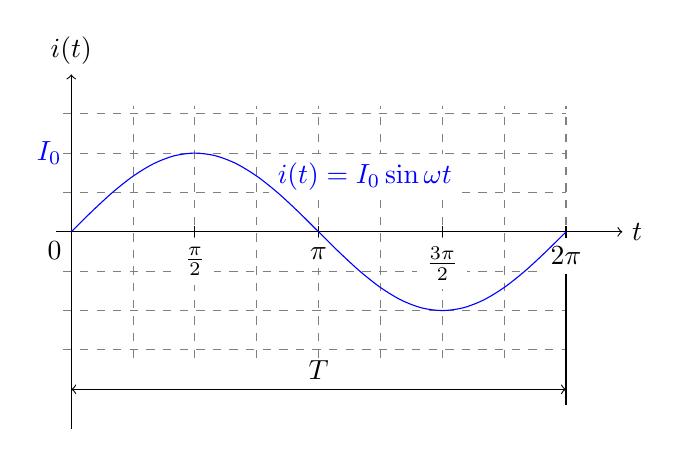
\begin{tikzpicture}[domain=0:2*pi] 
         \draw[xstep=pi/4, ystep=0.5, dashed, color=gray] (-0.1,-1.6) grid (2*pi,1.6); 
         \draw[->] (-0.2,0) -- (7,0) node[right] {$t$}; 
         \draw[->] (0,-2.5) -- (0,2) node[above] {$i(t)$}; 
         % text 
         \node[below left](0,0){$0$};
         \node[left, color=blue] at (0,1.0) {$I_0$}; 
         % period
         \draw[<->] (0,-2) -- (pi,-2) node[above]{$T$} --(2*pi,-2);
         \draw (2*pi,-2.2) -- (2*pi,0); 
         \foreach \x/\xtext in {0.5*pi/\frac{\pi}{2} ,pi/\pi, 1.5*pi/\frac{3\pi}{2}, 2*pi/2\pi}
         \draw[shift={(\x,0)}] (0pt,2pt) -- (0pt,-2pt) node[below, fill=white] {$\xtext$};  
         \node[below right, color=blue, fill=white] at (2.5,1.0) {$i(t) = I_0\sin\omega t$};
         % function 
         \draw[color=blue, smooth]   plot (\x,{sin(\x r)}); 
       \end{tikzpicture}  
       \captionsetup{type=figure}   
       \captionof{figure}{}\label{MA:fig_Iav_exam}
    \par}
  
%\end{document}